%%%%%%%%%%%%%%%%%%%%%%%%%%%%%%%%%%%%%%%%%%%%%%%%%%%%%%%%%%%%%%%%%%%%%%%%%%%%%%%
% Decomposing Lexicon-Assisted Correction for Word-Level Handwritten Text
%            Recognition on IAM: Lexicon Coverage, Frequency Ranking and
%            Line Context (Aachen writer-disjoint)
% Authors: Nur Banu Oğur (corresponding), Rıdvan Dursun, Berhat Yeşilyurt
%          Dept. of Software Engineering, Sakarya University
% Template: IJPRAI (World Scientific, ws-ijprai.cls)
%
% The IEEEtran conference version of this paper is kept in paper_ieee.tex.
%
% SABLON KURALLARI (ws-ijprai.pdf, ijprai-2e paketi):
%   - Ozet 200 kelimeden kisa, atifsiz ve denklemsiz olmali.
%   - Anahtar kelimeler noktali virgulle ayrilir, nokta ile biter.
%   - Tablo basligi USTTE (	bl), sekil basligi ALTTA.
%   - Cizgiler 	oprule / \colrule / otrule -- booktabs YUKLENMEZ,
%     sinif kendi tanimlarini verir; graphicx'i de sinif yukler.
%   - Tek kolon duzen: figure* yok.
%   - Kaynakca alfabetik, ws-ijprai.bst ile; atiflar ust simge (overcite).
%   - Tablo \label'i 	bl{...\label{}} icinde olmali, disarida bolum
%     numarasini yakalar.
%
% MODEL NAMING (used consistently throughout the paper):
%   no augmentation           = zero-augmentation anchor (positive control)
%   CRNN-B                    = baseline optical model, conventional augmentation
%   + wide photometric / + elastic / + morphological = ablation variants
%   CRNN-G                    = all augmentations, lexicon-free (greedy CTC)
%   CRNN-LX (PROPOSED)        = CRNN-G + 239K lexicon + Kneser-Ney trigram (IAM+Brown)
%                               ranked with the system's own line context
%   "unigram prior"           = the earlier corrector (add-one IAM unigram, alpha=5),
%                               kept as the no-context reference (80.74)
%
% ALL NUMBERS: full IAM labels, Aachen writer-disjoint split, N_test = 20,310,
% six configurations trained from scratch on one machine with one code
% revision, scored in fp32 with cuDNN deterministic algorithms; the two
% endpoint configurations additionally with seeds 123 and 456
% (results/ablation_viterbi_seeds.json -> Table 3).
% Sources: results/ablation_viterbi.json (Table 2; Table 3 rows 10-13),
% results/ablation_lexicon5_all.json (Table 3 rows 1-5),
% results/ablation_trigram.json (Table 3 rows 5-9, oracle),
% results/paper_stats_trigram.json (per-word counts), results/brown_leakage.json,
% per-word predictions in results/preds_viterbi/ (final) and results/preds_det/
%%%%%%%%%%%%%%%%%%%%%%%%%%%%%%%%%%%%%%%%%%%%%%%%%%%%%%%%%%%%%%%%%%%%%%%%%%%%%%%

\documentclass{ws-ijprai}

\usepackage{xcolor}
\usepackage{url,overcite}
% ws-ijprai.cls already loads graphicx and defines \toprule/\colrule/\botrule;
% loading booktabs on top of it would override the publisher's rule widths.
\usepackage[verbose,hypertexnames=false]{hyperref}
\hypersetup{colorlinks=false,allbordercolors=blue,pdfborderstyle={/S/U/W 1}}

% The class prints "<date> <time> <jobname>" above every page (\wsdraftnote,
% called from \cropmarks). That is a compile stamp, not part of the layout.
\makeatletter
\def\wsdraftnote{}
\makeatother

% ---- Custom commands ------------------------------------------------------
\newcommand{\ours}{CRNN-LX}            % proposed system (lexicon-extended)
\newcommand{\oursnolm}{CRNN-G}         % same optical model, greedy, no lexicon
\newcommand{\ourwa}{81.95\%}           % CRNN-LX: KN trigram, whole-line (Viterbi) decoding
\newcommand{\ourci}{[81.42\%, 82.48\%]}
\newcommand{\ourcer}{8.54\%}
\newcommand{\leftwa}{81.66\%}          % same model, trigram, left-to-right context only
\newcommand{\uniwa}{80.74\%}           % same model, unigram prior, no context
\newcommand{\unicer}{9.09\%}
\newcommand{\rawwa}{78.83\%}
\newcommand{\rawcer}{8.60\%}
\newcommand{\baselinewa}{81.64\%}      % CRNN-B, final corrector (Table 2 reference)
\newcommand{\deltawa}{0.32\,pp}        % CRNN-LX minus CRNN-B, final corrector
\newcommand{\anchordelta}{2.74}        % conventional pipeline removed, pp (final corrector)
\newcommand{\nsamples}{20{,}310}


\begin{document}

\markboth{N. B. O\u{g}ur, R. Dursun \& B. Ye\c{s}ilyurt}
         {Decomposing Lexicon-Assisted Correction for Handwritten Words}

%%%%%%%%%%%%%%%%%%%%% Publisher's area please ignore %%%%%%%%%%%%%%%
%
\catchline{}{}{}{}{}
%
%%%%%%%%%%%%%%%%%%%%%%%%%%%%%%%%%%%%%%%%%%%%%%%%%%%%%%%%%%%%%%%%%%%%

\title{Decomposing Lexicon-Assisted Correction for Word-Level\\
Handwritten Text Recognition on IAM: Lexicon Coverage,\\
Frequency Ranking and Line Context}

\author{Nur Banu O\u{g}ur\footnote{Corresponding author.}}

\address{Department of Software Engineering, Faculty of Computer and
Information Sciences,\\ Sakarya University, 54050 Sakarya, T\"urkiye\\
\email{nbogur@sakarya.edu.tr}}

\author{R\i dvan Dursun}

\address{Department of Software Engineering, Faculty of Computer and
Information Sciences,\\ Sakarya University, 54050 Sakarya, T\"urkiye\\
\email{ridvan.dursun@ogr.sakarya.edu.tr}}

\author{Berhat Ye\c{s}ilyurt}

\address{Department of Software Engineering, Faculty of Computer and
Information Sciences,\\ Sakarya University, 54050 Sakarya, T\"urkiye\\
\email{berhat.yesilyurt@ogr.sakarya.edu.tr}}

\maketitle

\begin{history}
\received{(Day Month Year)}
\revised{(Day Month Year)}
\accepted{(Day Month Year)}
\end{history}

\begin{abstract}
Handwriting varies strongly between writers, which makes word-level
recognition hard. We study it on the IAM database under the Aachen
writer-disjoint protocol, on all \nsamples\ test words. Our system,
\ours, is a convolutional-recurrent network trained from scratch,
followed by a lexicon-aware post-corrector that rescores candidates
with a Kneser--Ney trigram and decodes each text line jointly,
conditioning every word on the recognizer's own output for both of its
neighbours. Two questions are examined. The first concerns the
post-corrector, usually reported as a single language-model step.
Decomposing it reveals four ingredients with different jobs: lexicon
coverage decides the sign of the correction (a 7\,K-word training
vocabulary costs 2.4 points, a 239\,K-type English list gains 0.7);
the frequency prior that ranks candidates supplies most of the
magnitude (1.2 points); an external corpus adds 0.6 and line context
another 0.6, moving accuracy from \rawwa\ to \ourwa\ without raising
the character error rate. The second question is whether writing-aware
augmentation helps. Six configurations differing only in augmentation
show no detectable gain from elastic, morphological and wide
photometric transforms, whereas removing the conventional pipeline
beneath them costs \anchordelta\ points. Three seeds turn the
remaining gap into noise: it changes sign between them.
\end{abstract}

\keywords{Handwritten text recognition; lexicon-based post-correction;
Kneser--Ney trigram; line context; convolutional-recurrent neural
network; connectionist temporal classification; data augmentation;
ablation study.}

% ---- 1. Introduction ----------------------------------------------------
\section{Introduction}
\label{sec:intro}

Offline \emph{handwritten text recognition} (HTR) is the task of
converting a scanned image of handwriting into machine-readable text
without access to the pen trajectory. Depending on how the input is
segmented, an HTR system may operate on full pages, on text lines, or
--- as in this work --- on \emph{word} images. Word-level recognition
is the harder setting per sample, because the optical model sees one
crop at a time and cannot exploit the surrounding words to disambiguate
an unclear glyph. When the crops are cut from text lines, as in IAM,
that context is not lost entirely: the recognizer's own outputs for the
neighbouring crops are available, and whether a post-corrector can use
them is one of the questions examined here.

The IAM Handwriting Database~\cite{marti2002iam} is the standard
benchmark for English HTR, containing roughly 115\,000 word images from
657 writers. We adopt the partition released by RWTH Aachen
University~\cite{aachen_split} --- referred to as the \emph{Aachen
split} throughout this paper --- which guarantees that no writer
contributes to more than one of the training, validation and test
sets. This \emph{writer-disjoint} protocol is stricter than a random
split and is the realistic condition for deploying a recognizer on
handwriting it has never seen.

Modern recognizers are trained with the \emph{connectionist temporal
classification} (CTC) objective~\cite{graves2006connectionist}, which
removes the need for character-level alignment between the image and
its transcription. Two model families dominate: convolutional-recurrent
networks (CRNNs) trained with CTC~\cite{shi2017crnn, puigcerver2017,
bluche2017gated}, and attention-based sequence-to-sequence or
transformer encoders~\cite{kang2018convolve, michael2019evaluating}.
For a compact CRNN, two ingredients are commonly credited with closing
part of the gap to heavier models: data augmentation that reflects how
handwriting actually varies, and a lexical prior applied at or after
decoding. Both are widely used, but their individual contribution is
rarely measured under controlled conditions --- same data, same
architecture, same training schedule, same test set.

This paper provides such a measurement, and finds the two ingredients
unequal. On the augmentation side, the object of study is three
writing-aware transforms added on top of a conventional geometric and
photometric pipeline (rotation, translation, scaling, shear, brightness
and contrast jitter, Gaussian noise, gamma correction and random erasing;
Section~\ref{sec:aug}): \emph{elastic deformation}, which imitates the
small variations of a stroke from one writing to the next;
\emph{morphological perturbation}, which thins or thickens the strokes
as a fine or a broad pen would; and a \emph{widened photometric range},
which imitates lighter or darker ink and scans. Throughout the paper we
call these three the \emph{proposed transforms} and everything else the
\emph{conventional pipeline}. The label is ours rather than a standard:
there is no agreed set of routine augmentations for handwriting, and some
prior systems already treat elastic distortion as
one~\cite{dutta2018improving}. On the lexical side, the post-corrector
replaces a recognized word by a lexicon entry within a small edit
distance and ranks the candidates with a word-level language model; in
the proposed system that model is a Kneser--Ney trigram, and the words
of a text line are decoded jointly, so that each choice is conditioned
on the recognizer's own output for the neighbouring crops on both
sides. We
name the proposed system \ours\ (CRNN with lexicon-extended,
language-model-ranked post-correction) and its lexicon-free
counterpart \oursnolm; Table~\ref{tab:naming} defines the six
configurations compared. Our contributions are:

\begin{itemlist}
  \item \textbf{An anatomy of lexicon-assisted correction.} Holding the
        optical model fixed, we vary the post-correction lexicon, the
        language model that ranks the candidates, its training corpus
        and its context independently, which separates four effects
        that are usually reported as one. Coverage decides the sign:
        the training vocabulary alone \emph{hurts}, by 2.4 to 2.7
        percentage points (pp) on the five augmented models, while a
        general English list helps ($+0.3$ to $+0.7$\,pp). A unigram
        frequency prior then supplies most of the magnitude ($+1.1$ to
        $+1.3$\,pp), and its value grows with the lexicon, because a
        larger candidate set makes the ranking matter more. Replacing
        the prior by a trigram estimated on an external corpus adds
        $0.6$\,pp through the corpus and a further $0.6$\,pp through
        the line context --- read from the recognizer's own outputs,
        first from the left only and then from both sides by decoding
        the line jointly --- and brings the character error rate back
        to that of lexicon-free decoding. The complete corrector
        delivers $+3.1$\,pp, from \rawwa\ to \ourwa.
  \item \textbf{A controlled augmentation ablation with a positive
        control.} Six networks that differ only in the augmentation
        schedule are trained from scratch on the full Aachen training
        set and evaluated on the full test set. Elastic deformation,
        morphological perturbation and a widened photometric range
        change word accuracy by at most \deltawa, and none of those
        differences reaches the significance threshold ($p<0.01$) used
        throughout; removing the conventional pipeline underneath them
        costs \anchordelta\,pp at $p=1\times10^{-30}$. Repeating the two
        endpoint configurations with three seeds each shows why: the
        difference between them changes sign across seeds ($-0.49$ to
        $+0.78$\,pp) and the run-to-run spread of one configuration
        reaches $1.0$\,pp, several times the effect the transforms were
        expected to produce. These results are consistent with a
saturation effect rather than with an inability of the experimental
setup to detect augmentation-related improvements.
  \item \textbf{A methodological observation on elastic deformation.}
        The common parameterization --- normalized Gaussian-smoothed
        noise scaled by $\alpha\in[2,5]$ --- yields root-mean-square (RMS)
displacements of only 0.02--0.04 pixels per axis at the working
resolution and is effectively a no-op; we report the
        corrected parameterization we used and its effect.
  \item \textbf{A verified evaluation protocol and full release.}
        Writer-, prompt- and form-level disjointness of the split are
        checked programmatically; all \nsamples\ test words are used;
        code, split lists and per-word predictions are public.
\end{itemlist}

Section~\ref{sec:related} groups the related literature into four groups and positions our work within them.
Section~\ref{sec:method} describes the pipeline of
Fig.~\ref{fig:pipeline}. Section~\ref{sec:experiments} formalizes the
evaluation metrics and statistical tests.
Section~\ref{sec:results} reports the results,
Section~\ref{sec:discussion} analyzes them, and
Section~\ref{sec:conclusion} concludes.

% ---- 2. Related Work ----------------------------------------------------
\section{Related Work}
\label{sec:related}

We organize prior work into four groups according to how each relates
to ours: (i) \emph{recurrent CTC recognizers}, which share our optical
backbone but are almost always evaluated on text lines; (ii)
\emph{attention and transformer recognizers}, which target the same
word-level task as ours with a heavier decoding paradigm; (iii)
\emph{other word-level recognizers on IAM}, whose evaluation protocols
differ from ours; and (iv) \emph{lexical decoders}, which use a lexicon
or language model inside the decoding loop, whereas our post-corrector
applies it afterwards. For each group we state what we adopt and where
we differ.

\paragraph{Recurrent CTC recognizers.}
Graves and Schmidhuber~\cite{graves2008offline} introduced
multi-dimensional long short-term memory (LSTM) networks with CTC as
an early end-to-end offline recognizer. Puigcerver~\cite{puigcerver2017}
showed that a one-dimensional bidirectional LSTM (BiLSTM) stacked on a
convolutional neural network (CNN) feature extractor matches
multi-dimensional recurrence at a fraction of the cost, defining the
canonical CRNN baseline that our architecture follows. Bluche and
Messina~\cite{bluche2017gated} added gated convolutions, and Flor et
al.~\cite{flor2020htrflor} combined a CNN with a bidirectional gated
recurrent unit (BGRU) and a language-model pipeline. Wigington et
al.~\cite{wigington2017data} studied augmentation for CNN-LSTM
recognizers and reported gains from combined transforms on IAM lines.
We adopt the CRNN backbone unchanged; our contribution lies in
measuring, rather than assuming, the effect of the augmentation and of
the lexical prior.

\paragraph{Attention and transformer recognizers.}
Sueiras et al.~\cite{sueiras2018offline} and Kang et
al.~\cite{kang2018convolve} introduced sequence-to-sequence
recognizers with content-based attention for isolated IAM words.
Kang et al.~\cite{kang2021candidate} later integrated a language model
into the decoder itself through candidate fusion, and Kass and
Vats~\cite{kass2022attentionhtr} combined a residual-network (ResNet)
encoder,
attention decoding and transfer learning from scene-text corpora,
reporting the strongest word-level accuracy on the Aachen split that
we are aware of. These four systems share our task, metric and split
and are listed in Section~\ref{sec:results}. Transformer
architectures such as TrOCR~\cite{li2023trocr} have since lowered
line-level error rates further, but require pre-training on hundreds
of millions of synthetic lines. Multimodal large language models have
also been benchmarked on IAM~\cite{crosilla2025llmhtr}; those systems
operate on full pages and rely on proprietary pre-training corpora, so
they are not comparable to a from-scratch word recognizer.

\paragraph{Other word-level recognizers on IAM.}
Dutta et al.~\cite{dutta2018improving} improved a CNN--recurrent
neural network (RNN) hybrid with synthetic pre-training, slant
normalization and test-time augmentation and report a 12.61\%
unconstrained word error rate on IAM words evaluated without
punctuation or letter case, a setting not on the same footing as a
case-sensitive recognizer trained from scratch. Rajesh et
al.~\cite{rajesh2022hwrcnet} re-trained that CNN--RNN together with
their own HWRCNet, a CNN--BiLSTM operating in the JPEG discrete cosine
transform (DCT) domain, on a random 95:5 partition of IAM and obtained
77.14\% and 80.08\% strict word accuracy on uncompressed images; we
note that their headline figure of 89.05\% is \emph{word accuracy with
flexibility} of two edit operations rather than strict accuracy.
Taking a different route altogether, Mondal et
al.~\cite{mondal2022yolo} recognize IAM words lexicon-free by detecting
individual characters with a YOLOv3 object detector, trained on only
1\,200 word images, and report a 29.21\% word error rate on 30\,000
randomly selected test words. All three systems use partitions of IAM
other than ours, a point we return to below.

\paragraph{Lexical decoders.}
Most systems that exploit a vocabulary do so while decoding. Word beam
search (WBS)~\cite{scheidl2018wbs} injects a dictionary constraint
directly into CTC beam search, so that only lexicon words can be
produced; candidate fusion~\cite{kang2021candidate} feeds a language
model's proposals into an attention decoder; and Flor et
al.~\cite{flor2020htrflor} couple the optical model to a
language-model pipeline. In all of these the lexical knowledge is part
of decoding and cannot be varied without re-decoding or retraining. We
instead apply it \emph{after} greedy decoding, which lets us swap the
lexicon, the language model, its corpus and its context independently
while the optical hypotheses stay fixed. That is the property on which
the decomposition of Section~\ref{sec:res-lex} rests. The language
model itself is standard: an interpolated Kneser--Ney
$n$-gram~\cite{kneser1995improved, chen1999empirical}, the usual
smoothing for word $n$-gram models. What differs is where its context
comes from: a line-level decoder reads the preceding words off the same
image, whereas our corrector reads them off the recognizer's outputs
for the neighbouring word crops.

\paragraph{Positioning.}
Of the word-level systems above, only the attention-based recognizers
of Sueiras et al.~\cite{sueiras2018offline}, Kang et
al.~\cite{kang2018convolve, kang2021candidate} and Kass and
Vats~\cite{kass2022attentionhtr} are evaluated on the Aachen
writer-disjoint partition that we use; the CRNN-family results of
Rajesh et al.~\cite{rajesh2022hwrcnet} and the detector of Mondal et
al.~\cite{mondal2022yolo} use their own random partitions of IAM.
Comparisons across protocols are indicative only; the controlled
comparisons of this paper are those between our own configurations.

% ---- 3. Method ----------------------------------------------------------
\section{Proposed System}
\label{sec:method}

Fig.~\ref{fig:pipeline} shows the complete processing chain, from the
raw IAM word crops to the reported metrics, and marks the two stages
whose effect this paper measures.

\begin{figure}[th]
\centerline{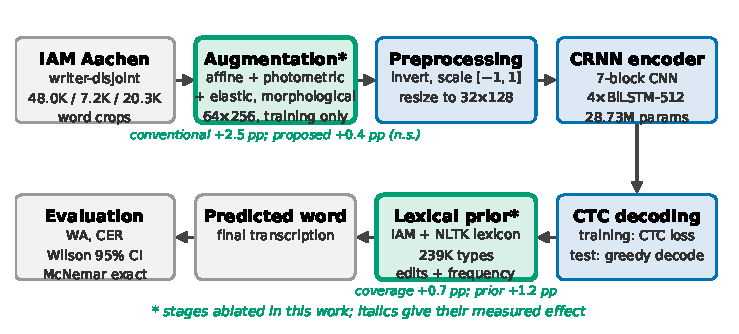
\includegraphics[width=\textwidth]{figures/fig0_pipeline.pdf}}
\vspace*{8pt}
\caption{Overview of \ours. Word crops are augmented (training only),
normalized, encoded by a CRNN and decoded with CTC; the decoded string
is then corrected against a 239\,K-type lexicon, the candidates of all
words on a text line being chosen jointly under a Kneser--Ney trigram,
so that each word is conditioned on the system's own output for its
neighbours. The two outlined
stages are the ones varied in the ablations, and each carries the
effects measured for it. The evaluation stage reports
word accuracy (WA), character error rate (CER) and Wilson confidence
intervals (CI), all defined formally in
Section~\ref{sec:experiments}.}
\label{fig:pipeline}
\alttext{Block diagram of the recognition pipeline, from the IAM Aachen
word crops through augmentation, preprocessing, the CRNN encoder, CTC
decoding and the lexicon post-corrector with trigram and line context
to evaluation. The two ablated stages are outlined and annotated with
their measured effects.}
\end{figure}

\subsection{Data and Protocol}
\label{sec:dataset}
We use the word-level IAM partition of the Aachen
split~\cite{aachen_split}: 747 training forms, 116 validation forms
and 336 test forms with disjoint writer sets (283, 55 and 161 writers
respectively). Following common practice, only word crops whose
segmentation is flagged \texttt{ok} are retained. Five validation
forms whose prompt text also occurs in the test set were removed from
the validation partition so that checkpoint selection is independent
of the test prompts; the test partition is used exactly as published.
This yields 47\,997 training words (two IAM image files are empty and
are skipped), 7\,205 validation words from 111 forms, and \nsamples\
test words from all 336 test forms. Writer, prompt and form
disjointness between the three partitions, as well as the integrity of
every record and image, are verified by a script distributed with the
code. The label alphabet contains 78 symbols (upper- and lower-case
Latin letters, digits and punctuation), plus the CTC blank.

\subsection{Model Naming}
\label{sec:naming}
Table~\ref{tab:naming} lists every configuration evaluated. All six
share the optical model of Section~\ref{sec:model}, the training
schedule and the post-corrector of Section~\ref{sec:trigram}; they
differ only in the augmentation applied during training. \oursnolm\ is
the fully augmented optical model decoded greedily, without any
lexicon; \ours\ is that same model followed by the extended-lexicon
post-corrector of Section~\ref{sec:trigram} with the trigram and
whole-line decoding, and is the configuration we propose. The suffixes denote the
post-processing rather than the augmentation, which turns out not to
matter (Section~\ref{sec:res-aug}). The first row is
the zero-augmentation anchor: it has the conventional pipeline switched
off as well, and exists so that the ablation can distinguish ``the
proposed transforms add nothing'' from ``this pipeline cannot detect
augmentation at all''.

\begin{table}[th]
\tbl{Configurations compared. All use the same 28.73\,M-parameter
network, the same schedule and the same post-corrector. The rows are
cumulative: elastic and morphological perturbation are each added on
top of the widened photometric range. Conventional: the pipeline listed
in Section~\ref{sec:aug}.\label{tab:naming}}
{\begin{tabular}{lcccc}
\toprule
Name & Conventional & Wide photometric & Elastic & Morphological \\
\colrule
no augmentation            & no  & no  & no  & no  \\
CRNN-B (baseline)          & yes & no  & no  & no  \\
$+$ wide photometric       & yes & yes & no  & no  \\
$+$ elastic                & yes & yes & yes & no  \\
$+$ morphological          & yes & yes & no  & yes \\
\textbf{\ours} (proposed)  & yes & yes & yes & yes \\
\botrule
\end{tabular}}
\end{table}

\subsection{Optical Model}
\label{sec:model}
The encoder is a seven-block convolutional feature extractor that
collapses the input to a single row of 512-dimensional frames,
followed by a four-layer bidirectional LSTM with 512 hidden units and
a linear projection onto the 79 output classes; the network has
28.73\,M parameters. Inputs are grayscale crops resized to
$32\times128$, inverted so that ink is high-valued, and scaled to
$[-1,1]$. The network is trained with the CTC
objective~\cite{graves2006connectionist} using AdamW with learning
rate $\eta=7\times10^{-4}$ and weight decay $10^{-5}$, five warm-up
epochs followed by cosine decay, mixed precision, and batches of 128,
for at most 100 epochs. Training stops when neither the validation loss nor the validation
word accuracy has improved for 15 epochs, and the checkpoint with the
best validation word accuracy is evaluated once on the test set. The
validation accuracy used for early stopping and checkpoint selection is
computed with the extended lexicon and the unigram prior of
Section~\ref{sec:trigram}, identically for all six configurations; the
trigram corrector is applied only afterwards, to the frozen checkpoints,
so that it never influences which weights are selected.

\subsection{Augmentation}
\label{sec:aug}
The baseline (CRNN-B) uses what we call the conventional pipeline: rotation
($\pm7^\circ$), translation ($\pm5\%$), scaling ($0.9$--$1.1$), shear
($\pm5^\circ$), brightness and contrast jitter ($0.85$--$1.15$),
Gaussian noise ($\sigma=0.03$), gamma correction ($0.80$--$1.20$) and
random erasing. The proposed transforms, which the ablation variants add
cumulatively, are:

\begin{itemlist}
  \item \textbf{Wide photometric range.} Brightness and contrast
        $0.70$--$1.35$, gamma $0.70$--$1.30$, noise $\sigma=0.05$.
  \item \textbf{Elastic deformation} (probability $0.5$). A random
        displacement field is smoothed with a Gaussian kernel whose
        width is $8\%$ of the larger image side, rescaled to unit RMS,
        and multiplied by an amplitude drawn uniformly from $[1,3]$
        pixels; the crop is warped accordingly. The unit-RMS
        normalization is essential: the frequently used variant that
        multiplies the \emph{unnormalized} blurred noise by
        $\alpha\in[2,5]$~\cite{simard2003best} produces, at the $64\times256$
working resolution, per-axis RMS displacements of only 0.02--0.04
pixels (never more than 0.19\,px), i.e.\ it leaves the image visually
and numerically unchanged. Our own earlier implementation had this property.
  \item \textbf{Morphological perturbation} (probability $0.15$). The
crop is eroded or dilated, with equal probability, by a $2\times2$
kernel, reproducing the difference between a fine and a broad nib.
\end{itemlist}

Fig.~\ref{fig:augmentation} illustrates the transforms. All
augmentation is applied on the graphics processing unit (GPU) to whole
batches at a working
resolution of $64\times256$ pixels (the median IAM word height is
68\,px), with independent random parameters per sample, before the
final resize to $32\times128$; the same code path is used by all six
configurations. The zero-augmentation anchor bypasses that code path
entirely, so its crops reach the network with preprocessing only.

\begin{figure}[th]
\centerline{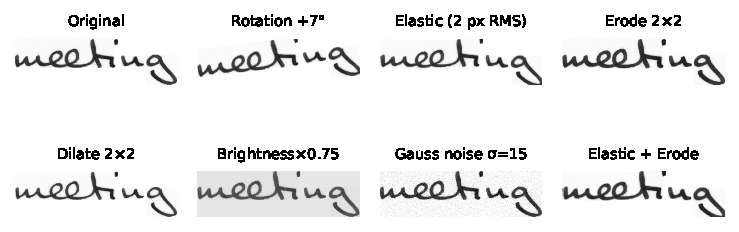
\includegraphics[width=\textwidth]{figures/fig1_augmentation_grid.pdf}}
\vspace*{8pt}
\caption{Augmentation transforms on a training crop. The elastic panel
uses the corrected amplitude (2\,px RMS); the last panel shows the
compound elastic$+$morphological effect.}
\label{fig:augmentation}
\alttext{Eight versions of the same handwritten word crop, showing the original and seven augmentation transforms applied to it.}
\end{figure}

\subsection{Lexicon-Extended Post-Correction with Line Context}
\label{sec:trigram}
After greedy CTC decoding, each hypothesis is checked against a closed
lexicon. If the hypothesis (case-insensitively) is in the lexicon it is
accepted unchanged; otherwise it is replaced by the best-scoring
lexicon entry within a Levenshtein distance of 1 (words of up to four
characters) or 2 (longer words). On the test set 3\,260 hypotheses
(16.1\%) fall outside the extended lexicon, and 2\,939 of them have at
least one candidate within that distance; the other words pass through
unchanged, so everything the corrector can gain or lose is decided
among those 2\,939. A candidate $c$ at edit distance $d$ from the hypothesis is
scored as
\begin{equation}
s(c) \;=\; \log P(c \mid h_1, h_2) \;-\; \alpha\, d ,
\label{eq:score}
\end{equation}
where $P$ is a word-level language model, $h_1 h_2$ are the two words
that precede the hypothesis on its text line, and $\alpha$ is an edit
penalty selected on the validation partition. The lexicon, the language
model and the way the line is decoded are the variables of interest,
and Section~\ref{sec:res-lex} varies them one at a time with the
optical model held fixed.

\paragraph{Lexicon.}
The \emph{training lexicon} consists of the 7\,173 word types of the
training transcriptions; the \emph{extended lexicon} adds the Natural
Language Toolkit (NLTK) English word list, giving 239\,126 types.
Measured on the test transcriptions, the training lexicon covers
84.8\% of the test tokens and the extended lexicon 93.9\%; the
remaining tokens are proper nouns, inflected forms absent from both
lists, and punctuation-bearing strings.

\paragraph{Language model.}
Two models are compared. The \emph{unigram frequency prior} ignores the
context: it is the add-one-smoothed relative frequency of $c$ among the
47\,999 tokens of the training transcriptions, with $\alpha=5$. It is the corrector of an
earlier version of this work and serves as the reference. The
\emph{trigram with line context}, used by \ours, is an interpolated
Kneser--Ney trigram~\cite{chen1999empirical} with absolute discount
$0.75$ and an additive floor over the lexicon vocabulary so that every
candidate keeps a positive probability; an unseen trigram context
degrades to the bigram and then to the unigram estimate. It is estimated
on the same 47\,999 tokens, read as text lines, and, in the proposed
configuration, additionally on the Brown corpus~\cite{francis1979brown}
(57\,340 sentences, 1.16\,M tokens). Tokens are case-sensitive and
punctuation marks are kept as tokens, matching the IAM transcriptions.

\paragraph{Context.}
IAM word crops are cut from text lines and keep their position on the
line, so the recognizer's outputs for the neighbouring crops are
available at test time. The context in Eq.~(\ref{eq:score}) is the
system's \emph{own output} for the neighbouring word crops of the same
line --- never their reference transcription. A line is a contiguous
run of crops; the run is broken, and the context reset, wherever a
crop is missing from the split (crops whose segmentation IAM flags as
not \texttt{ok}). On the test set 88.5\% of the words have a preceding
crop. The optical model still sees one isolated crop at a time; only
the post-corrector reads across the line, and the no-context figure is
reported alongside for the setting in which words are genuinely
isolated.

\paragraph{Decoding the line.}
Two decoders are compared. The \emph{left-to-right} decoder corrects
the words of a line in reading order, scoring each by
Eq.~(\ref{eq:score}) with $h_1 h_2$ set to its own two previous
outputs, so a word is conditioned on its left neighbours only. The
\emph{whole-line} decoder, used by \ours, instead chooses the word
sequence $w_1\ldots w_n$ of the line that maximizes
$\sum_i [\log P(w_i \mid w_{i-2}, w_{i-1}) - \alpha\, d_i]$ over all
combinations of candidates, by exact second-order Viterbi search; since
$w_i$ also enters the terms of $w_{i+1}$ and $w_{i+2}$, every choice
is conditioned on the words to its left \emph{and} right. Each
out-of-lexicon hypothesis contributes a column of its candidates (at
most the ten with the best context-free score); an in-lexicon
hypothesis contributes only itself. Two options of the whole-line
decoder are tested and selected on validation: whether an
out-of-lexicon hypothesis may also stay as it is, as a candidate at
distance zero with the model's unseen-word floor probability, so that a
correct word absent from the lexicon (a proper noun, an inflection)
survives when the line supports it (\emph{keep-OOV}); and whether an
in-lexicon hypothesis may be replaced by a lexicon neighbour at
distance one, so that real-word errors such as \emph{form}/\emph{from}
become correctable (\emph{real-word}). For the whole-line decoder
$\alpha$ is selected from $\{1,2,3,4,5,7,10,15,20,30\}$, a wider grid
than the $\{3,5,7,10\}$ of the left-to-right decoder because the line
objective shifts the useful range. Every selection --- $\alpha$, the
options, the decoder --- is made on the validation writers and applied
once to the test set.

\paragraph{External corpus.}
The IAM prompts were taken from the LOB corpus; Brown is a different
corpus of the same design (American English, 1961), so overlap has to
be measured rather than assumed. Of the word 5-grams on the test lines
0.63\% occur verbatim in Brown, of the 6-grams 0.11\%, of the 8-grams
none; the longest shared sequence is seven words and the shared strings
are idioms (\emph{in spite of the fact that}, \emph{on the other
hand}). The same check against the IAM training lines gives 0.06\% and
0\%. The corpus therefore supplies English word statistics, not the
test text, and the corrector never sees an IAM test transcription.

% ---- 4. Experimental Setup ----------------------------------------------
\section{Experimental Setup}
\label{sec:experiments}

\subsection{Evaluation Metrics}
Let $\mathcal{T}=\{(\hat{y}_i, y_i)\}_{i=1}^{N}$ be the set of
$N=\nsamples$ predicted/reference word pairs. \emph{Word accuracy}
(WA) is the exact-match rate
\begin{equation}
\mathrm{WA} \;=\; \frac{1}{N}\sum_{i=1}^{N}
      \mathbb{1}\!\left[\hat{y}_i = y_i\right],
\label{eq:wa}
\end{equation}
and the word error rate (WER) follows as
$\mathrm{WER}=1-\mathrm{WA}$. The \emph{character error rate} (CER)
aggregates Levenshtein distances $d(\cdot,\cdot)$ over the corpus,
\begin{equation}
\mathrm{CER} \;=\;
  \frac{\sum_{i=1}^{N} d(\hat{y}_i, y_i)}
       {\sum_{i=1}^{N} |y_i|},
\label{eq:cer}
\end{equation}
so that a single badly recognized long word cannot dominate the score.

\subsection{Confidence Intervals}
Because WA is a proportion estimated on a finite test set, we report
Wilson 95\% confidence intervals (CIs) rather than
normal-approximation intervals, which are unreliable near the
boundaries. For $k$ correct predictions out of $N$ and $z=1.96$,
\begin{equation}
\mathrm{CI}_{95} =
\frac{\hat{p}+\frac{z^{2}}{2N} \pm
      z\sqrt{\frac{\hat{p}(1-\hat{p})}{N}+\frac{z^{2}}{4N^{2}}}}
     {1+\frac{z^{2}}{N}},
\qquad \hat{p}=\frac{k}{N}.
\label{eq:wilson}
\end{equation}
With $N=\nsamples$ the half-width of the interval is about 0.55\,pp.

\subsection{Significance Testing}
Two systems evaluated on the same test set produce paired outcomes, so
we use the exact McNemar test. Let $b$ be the number of samples that
the first system recognizes correctly and the second does not, and $c$
the converse. Under the null hypothesis the discordant pairs are
distributed $\mathrm{Bin}(b+c,\,\tfrac{1}{2})$, giving the two-sided
$p$-value
\begin{equation}
p \;=\; \min\!\left(1,\;
   2\sum_{i=0}^{\min(b,c)} \binom{b+c}{i} 2^{-(b+c)}\right).
\label{eq:mcnemar}
\end{equation}
We treat $p<0.01$ as significant.

\subsection{Reproducibility}
All six configurations were trained on the same machine (one NVIDIA
GeForce RTX~4070 Laptop GPU with 8\,GB, PyTorch~2.7.1 with CUDA~11.8,
Python~3.13) from the same code revision, with seed 42, at 35--75\,s per
epoch; a configuration takes roughly one hour. The two endpoint
configurations, CRNN-B and \ours, were additionally re-trained with
seeds 123 and 456 by one of the authors on a different machine (one
NVIDIA T4 through a hosted notebook service), from the same code
revision, the same split files --- verified byte-identical apart from
line endings --- and the same hyperparameters; only the seed and the
hardware differ. The four intermediate configurations were trained
once, and differences smaller than the confidence interval are not
interpreted. Every number
reported below comes from evaluation passes in single precision with
cuDNN restricted to its deterministic algorithms, in which the six
optical models and all post-corrections are scored against identical
greedy hypotheses, model by model; two separate processes produce byte-identical
hypotheses for all \nsamples\ test words. Without that restriction
single precision was reproducible within a process but one word
changed between processes, and mixed-precision inference shifted 2
words between runs (0.01\,pp). The post-corrector is deterministic: candidates are
enumerated in a fixed order (shorter first, then lexicographic), ties
keep the first candidate, and the output does not depend on the order
in which lines are processed. Two numerical self-tests, distributed
with the code, confirm that the trigram's conditional distributions sum
to one over the 271\,303-type vocabulary for seen and unseen contexts,
and that the whole-line decoder returns the same optimum as an
exhaustive search over all candidate combinations on 400 random line
layouts. Code, split
definitions, the split-verification script, the language-model and
leakage-check scripts, per-word predictions and evaluation scripts are
available at
\url{https://github.com/Ridvan013/CRNN-Handwriting-Recognition}
(branch \texttt{feature/aachen-v3-extended-trigram}); the trained
weights exceed the repository file-size limit and are distributed
separately.

% ---- 5. Results ---------------------------------------------------------
\section{Results}
\label{sec:results}

\subsection{Augmentation Ablation}
\label{sec:res-aug}

Table~\ref{tab:main} is the central result, and it separates into two
layers.

The conventional pipeline matters. Removing it costs \anchordelta\,pp
(81.64 to 78.90\%) and $1.69$\,pp of character error rate; 1\,457
words are recognized only by the baseline against 900 only by the
anchor, and the exact McNemar test rejects equality at
$p=1\times10^{-30}$. Without a lexicon the same comparison is wider
still, 78.77 against 74.33\% ($-4.44$\,pp), so part of the weaker
optical model is masked by the post-corrector.

The proposed transforms do not provide a statistically detectable
improvement. The five
configurations that keep the conventional pipeline reach
81.64--81.95\%, and none differs from the baseline at the $p<0.01$
threshold of Section~\ref{sec:experiments}. The full scheme (\ours) is
nominally the best, \deltawa\ above the baseline ($p=0.132$), which is
within one confidence-interval half-width; elastic perturbation alone
gives $p=0.182$, morphological perturbation $0.466$ and the widened
photometric range $0.712$. The comparison is also sensitive to the
post-corrector, which is why we report it under all three: scored with
the unigram prior the same two optical models differ by $0.38$\,pp at
$p=0.060$, with the left-to-right trigram by $0.44$\,pp at $p=0.025$,
and with the whole-line decoder by \deltawa\ at $p=0.131$ --- the same
sign every time, never below the threshold.

Three seeds resolve the question, and they resolve it against the
transforms. Table~\ref{tab:seeds} repeats CRNN-B and \ours\ with
seeds 123 and 456. The difference between the two changes sign:
\ours\ is $0.32$\,pp above CRNN-B at seed 42, $0.49$\,pp
\emph{below} it at seed 123 and $0.78$\,pp above it at seed 456. Two
of the three per-seed comparisons would be declared significant at the
$0.05$ level --- in opposite directions ($p=0.024$ and
$p=4\times10^{-4}$). Averaged over the three seeds the difference is
$+0.20\pm0.64$\,pp (paired $t(2)=0.54$, $p=0.64$), and one unchanged
configuration spans a full point on its own (\ours: 81.43--82.44\%).
The run-to-run spread is therefore several times the effect under
study, which is why we report the augmentation comparison as
unresolved rather than as a small gain; the conventional pipeline, at
\anchordelta\,pp, sits an order of magnitude above that noise floor
and is untouched by the argument. A practical consequence is that a
single-seed McNemar test on 20\,K words can report a significant
augmentation effect of either sign, so the per-configuration
$p$-values of Table~\ref{tab:main} should be read as descriptive.
Because the configurations are nested,
Table~\ref{tab:main} reports two differences: $\Delta_{\mathrm{B}}$
against the baseline CRNN-B, and $\Delta_{\mathrm{P}}$ against the
$+$wide photometric configuration on which elastic and morphological
perturbation are built, which isolates each transform. By
$\Delta_{\mathrm{P}}$, elastic perturbation adds $0.21$\,pp,
morphological perturbation $0.07$\,pp and the two together
$0.23$\,pp; the widened photometric range itself adds $0.08$\,pp,
which is why $\Delta_{\mathrm{B}}$ is larger by that amount ($+0.29$,
$+0.16$ and $+0.32$\,pp). On the per-word level these five disagree on
3\,773 words (18.6\%), yet the disagreements largely cancel: for the
baseline--\ours\ pair, 841 words are recognized only by the baseline
and 904 only by \ours. Among configurations that
already augment, the choice of transform changes \emph{which} words are
recognized far more than \emph{how many}.

\begin{table}[th]
\tbl{Augmentation ablation on the Aachen writer-disjoint test set
($N=\nsamples$). All rows share the network, schedule and
post-corrector (239\,K lexicon, Kneser--Ney trigram on IAM$+$Brown,
whole-line decoding with keep-OOV; the edit penalty, selected on
validation for each model separately, is $\alpha=2$ or $3$).
$\Delta_{\mathrm{B}}$ is the difference in WA to
CRNN-B and $\Delta_{\mathrm{P}}$ the difference to the $+$wide
photometric configuration on which elastic and morphological
perturbation are added; both are computed from unrounded accuracies.
$p$ is the exact McNemar test against CRNN-B on per-word outcomes. The
first row is the zero-augmentation anchor and acts as a positive
control. Best validation WA and the epoch at which it was reached are
given for reference (validation: 7\,205 words, 55
writers).\label{tab:main}}
{\begin{tabular}{lccccccc}
\toprule
Configuration & WA (\%) & CER (\%) & Wilson 95\% CI & $\Delta_{\mathrm{B}}$ & $\Delta_{\mathrm{P}}$ & $p$ & best val WA (ep.) \\
\colrule
no augmentation        & 78.90 & 10.52 & [78.33,\,79.45] & $-2.74$ & ---     & $1\!\times\!10^{-30}$ & 82.57 (38) \\
CRNN-B (baseline)      & 81.64 & 8.83  & [81.10,\,82.17] & (ref.)  & ---     & (ref.) & 84.61 (87) \\
$+$ wide photometric   & 81.72 & 8.39  & [81.19,\,82.25] & $+0.08$ & (ref.)  & 0.712  & 84.34 (76) \\
$+$ elastic            & 81.93 & \textbf{8.21} & [81.39,\,82.45] & $+0.29$ & $+0.21$ & 0.182  & 84.69 (77) \\
$+$ morphological      & 81.80 & 8.25  & [81.26,\,82.32] & $+0.16$ & $+0.07$ & 0.466  & 84.58 (84) \\
\textbf{\ours} (all)   & \textbf{81.95} & 8.54 & [81.42,\,82.48] & $+0.32$ & $+0.23$ & 0.132 & 84.77 (70) \\
\botrule
\end{tabular}}
\end{table}

\begin{table}[th]
\tbl{Seed repeats of the two endpoint configurations, scored with the
corrector of Table~\ref{tab:main} ($N=\nsamples$). Seed 42 is the run
reported throughout the paper; seeds 123 and 456 differ from it only in
the seed and in the machine they were trained on
(Section~\ref{sec:experiments}). $\Delta$ is \ours\ minus CRNN-B
within a seed and $p$ the exact McNemar test on that pair; the two
differences that reach $p<0.05$ have opposite signs.\label{tab:seeds}}
{\begin{tabular}{lccccc}
\toprule
Seed & CRNN-B & \ours & $\Delta$ & $p$ & CER: CRNN-B / \ours \\
     & WA (\%) & WA (\%) & (pp) & & (\%) \\
\colrule
42 & 81.64 & 81.95 & $+0.32$ & 0.132 & 8.83 / 8.54 \\
123 & 81.93 & 81.43 & $-0.49$ & 0.024 & 8.20 / 8.91 \\
456 & 81.66 & 82.44 & $+0.78$ & $4\!\times\!10^{-4}$ & 8.53 / 8.28 \\
\colrule
mean $\pm$ SD & $81.74\pm0.16$ & $81.94\pm0.50$ & $+0.20\pm0.64$ & 0.644\tabmark{a} & $8.52\pm0.32$ / $8.57\pm0.32$ \\
\botrule
\end{tabular}}
\begin{tabfootnote}
\tabmark{a} Paired $t$ test on the three per-seed differences,
$t(2)=0.54$; the $p$ values above it are per-seed McNemar tests.
\end{tabfootnote}
\end{table}

Fig.~\ref{fig:curves} shows the mechanism. The anchor separates from
the rest early: by epoch 53 its training loss is down to 0.018, where
the augmented runs are still at 0.056--0.070, while its validation
accuracy peaks at 82.57\% at epoch 38 and early stopping ends the run
at epoch 53. It fits the training set far more tightly and generalizes
worse: its validation loss ends at 0.46 against 0.32--0.37 for the
augmented runs. Those five keep improving to epoch 70--87 and converge
to a plateau of 84.3--84.8\% validation accuracy, and among them the
curves are indistinguishable after the first fifteen epochs; their
training losses differ a little (the fully augmented model fits the
training set least tightly, as a regularizer should), but the spread
that reaches validation accuracy is only 0.4\,pp. With 47\,997 training
words from 283 writers, the conventional pipeline already covers the
variability that the proposed transforms simulate.

\begin{figure}[th]
\centerline{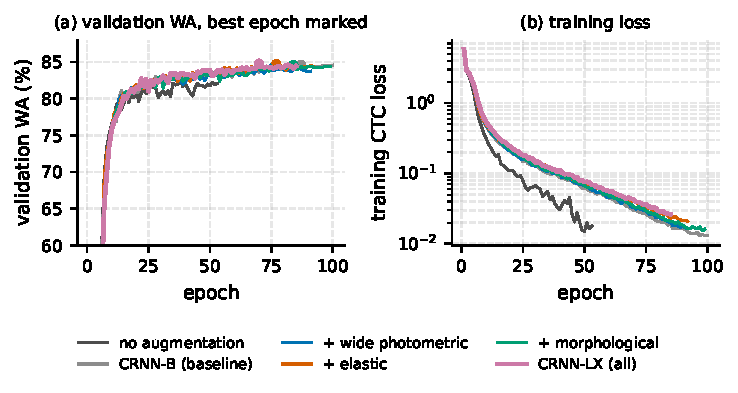
\includegraphics[width=\textwidth]{figures/fig2_training_curves.pdf}}
\vspace*{8pt}
\caption{Training dynamics of the six configurations: (a) validation
word accuracy with the best epoch marked, (b) training CTC loss. The
zero-augmentation anchor reaches the lowest training loss and the
lowest validation accuracy; the five augmented curves coincide.}
\label{fig:curves}
\alttext{Two line charts over training epochs: validation word accuracy on the left and training CTC loss on the right, one curve per configuration.}
\end{figure}

\subsection{Lexicon Ablation}
\label{sec:res-lex}

Table~\ref{tab:lexicon} holds the optical model fixed (\ours, best
checkpoint) and varies only what happens after greedy decoding. The
effect is an order of magnitude larger than that of the augmentation.
The corrector has four ingredients --- the lexicon a hypothesis is
tested against, the language model that ranks the candidates within
edit distance, the corpus that model is estimated on, and the context
it is given --- and the table varies them one at a time, so that rows
2 and 4 isolate coverage at fixed ranking, rows 2$\to$3 and 4$\to$5
isolate the frequency prior at a fixed lexicon, rows 5--9 isolate the
corpus and the left context at a fixed lexicon, and rows 9--13 vary
only how the line is decoded.

Coverage decides the sign. Against the training vocabulary alone,
accuracy \emph{falls} from \rawwa\ to 76.42\%: hypotheses that are
valid English words absent from the 7\,K training list --- 15\% of
the test tokens --- are forced onto the nearest training word, and most
of these substitutions are wrong. Replacing that list with 239\,K
types, which covers 94\% of the test tokens, turns the same
$-2.41$\,pp into $+0.68$\,pp (76.42 to 79.51\%, a swing of 3.09\,pp
at identical ranking).

The frequency prior supplies most of the magnitude, and its value
grows with the lexicon. On the 7\,K list it is worth $+0.62$\,pp
(76.42 to 77.04\%); on the 239\,K list, $+1.23$\,pp (79.51 to
\uniwa). Fig.~\ref{fig:lexdecomp}(a) shows both effects at once. The
reason is combinatorial rather than linguistic: a larger lexicon puts
more entries within the same edit distance of a hypothesis, so the
choice among equidistant candidates --- which is exactly what the prior
makes --- decides more cases, and Section~\ref{sec:disc-lex} takes the
argument further. Neither ingredient alone reaches the $+1.91$\,pp of
the unigram corrector.

The corpus and the context supply the rest
(Fig.~\ref{fig:lexdecomp}(b)). Rows 5--9 keep the extended lexicon and
change only the language model of Eq.~(\ref{eq:score}). Replacing the
add-one prior by a Kneser--Ney unigram estimated on the same IAM text
changes nothing (\uniwa\ in both cases; 19 words gained, 18 lost), so
the smoothing is immaterial. Giving that model the line context, still
on IAM text alone, adds only $0.10$\,pp (80.84\%, $p=0.022$): 48\,K
tokens of training text rarely contain the context of a test word.
Adding the Brown corpus to the context-free model adds $+0.59$\,pp
(81.32\%, $p=9\times10^{-19}$; 155 words gained against 36 lost), and
the trigram with line context on the enlarged corpus adds a further
$+0.34$\,pp, reaching \leftwa\ ($p=1\times10^{-35}$ against the
unigram prior; 220 words gained against 32 lost). Decomposed in the
other order --- context first, corpus second --- the shares are
$+0.10$ and $+0.83$\,pp, so the two ingredients are not additive:
context is worth little until the corpus is large enough to have seen
it. Two diagnostics bound this step. Replacing the system's own
outputs by the reference transcriptions of the neighbouring crops (an
oracle, not a reportable system) gives 81.73\%, only $0.06$\,pp more,
so almost nothing is lost to the recognizer's own errors in the
context. And the edit penalty is not what carries the result:
$\alpha=7$ was selected on the validation set, but every value tried
($3$, $5$, $7$, $10$) gives between 81.43 and 81.66\% on the test set,
all above the unigram prior.

Decoding the line jointly adds the last step (rows 10--13). With the
same trigram, choosing all words of a line together instead of left to
right --- so that a word is also conditioned on what follows it ---
gains $0.11$\,pp (81.77\%, $p=0.026$; 56 words gained, 34 lost).
Allowing an out-of-lexicon hypothesis to survive as a candidate
(keep-OOV) gains a further $0.18$\,pp, reaching \ourwa\ ($p=0.032$
against the left-to-right decoder, 394 gained against 335 lost), and it
does so by making the corrector \emph{more} conservative: it now
replaces 1\,925 hypotheses instead of 2\,939, repairs 815 and breaks
181, where the left-to-right decoder repaired 1\,076 and broke 501.
Allowing real-word substitutions (row 12) reaches 81.94\% on the test
set with fewer but surer changes (141 gained, 86 lost, $p=3\times
10^{-4}$), but it scored below keep-OOV on the validation set and was
therefore not selected; the two options together (row 13) interact
badly, since a hypothesis that keeps itself at distance zero now
competes with real-word substitutions of its neighbours, and lose
$2.2$\,pp. The whole-line decoder with keep-OOV was selected on
validation and is the configuration of \ours; on the four other
augmented models of Table~\ref{tab:main} it gains $0.32$--$0.44$\,pp
over the left-to-right decoder ($p=0.002$--$0.034$), and $0.08$\,pp
($p=0.57$) on the zero-augmentation anchor, whose weaker hypotheses
give the line objective less to work with. In all, the corrector moves
\oursnolm\ from \rawwa\ to \ourwa: coverage $+0.7$, frequency prior
$+1.2$, corpus $+0.6$, line context $+0.6$\,pp.
The unigram pattern holds on the other four augmented optical models of
Table~\ref{tab:main}: the training lexicon costs 2.4--2.7\,pp, the
extended lexicon gains 0.3--0.7\,pp over lexicon-free decoding, the
prior adds a further 1.1--1.3\,pp, and the complete corrector gains
1.5--1.9\,pp. On the zero-augmentation anchor, whose greedy output is
4.4\,pp weaker, the ordering is unchanged but every effect is larger
and the complete corrector gains 3.54\,pp: the more the optical model
errs, the more a lexical prior has to repair.

\begin{table}[th]
\tbl{Post-correction ablation with the optical model fixed (\ours\
checkpoint, $N=\nsamples$). Each row applies a different
post-correction to the \emph{same} greedy hypotheses; lexicon,
language model, corpus, context and line decoding vary one at a time.
KN1/KN3: interpolated Kneser--Ney unigram/trigram; L$\to$R: the trigram
is given the system's own outputs for the two preceding crops of the
line; line: whole-line (Viterbi) decoding, conditioned on both
neighbours. Edit penalty $\alpha=5$ for the add-one prior; otherwise
selected on the validation set (5 for row 6, 7 for rows 7--9, 10 for
rows 10, 12 and 13, 2 for row 11). Rows 12 and 13 are reported for
completeness; they scored below row 11 on validation and were not
selected.\label{tab:lexicon}}
{\begin{tabular}{llrccc}
\toprule
Post-correction & Ranking (corpus) & Lexicon & WA (\%) & CER (\%) & Wilson 95\% CI \\
\colrule
none (\oursnolm, greedy CTC)              & ---                       & n/a      & 78.83 & 8.60 & [78.27,\,79.39] \\
training lexicon, edit distance only      & ---                       & 7\,173   & 76.42 & 11.19 & [75.83,\,76.99] \\
training lexicon $+$ frequency prior     & add-one unigram (IAM)     & 7\,173   & 77.04 & 10.94 & [76.46,\,77.61] \\
extended lexicon, edit distance only      & ---                       & 239\,126 & 79.51 & 9.71 & [78.95,\,80.06] \\
extended lexicon $+$ frequency prior     & add-one unigram (IAM)     & 239\,126 & 80.74 & 9.09 & [80.19,\,81.28] \\
extended lexicon $+$ KN1                  & KN1 (IAM)                 & 239\,126 & 80.74 & 9.09 & [80.20,\,81.28] \\
extended lexicon $+$ KN3, L$\to$R         & KN3 (IAM)                 & 239\,126 & 80.84 & 9.07 & [80.29,\,81.37] \\
extended lexicon $+$ KN1                  & KN1 (IAM$+$Brown)         & 239\,126 & 81.32 & 8.74 & [80.78,\,81.85] \\
extended lexicon $+$ KN3, L$\to$R         & KN3 (IAM$+$Brown)         & 239\,126 & 81.66 & 8.58 & [81.13,\,82.19] \\
extended lexicon $+$ KN3, line            & KN3 (IAM$+$Brown)         & 239\,126 & 81.77 & 8.54 & [81.24,\,82.30] \\
\textbf{extended lexicon $+$ KN3, line, keep-OOV} (\ours) & KN3 (IAM$+$Brown) & 239\,126 & \textbf{81.95} & 8.54 & [81.42,\,82.48] \\
extended lexicon $+$ KN3, line, real-word & KN3 (IAM$+$Brown)         & 239\,126 & 81.94 & \textbf{8.51} & [81.40,\,82.46] \\
extended lexicon $+$ KN3, line, keep-OOV $+$ real-word & KN3 (IAM$+$Brown) & 239\,126 & 79.71 & 8.42 & [79.16,\,80.26] \\
\botrule
\end{tabular}}
\end{table}

\begin{figure}[th]
\centerline{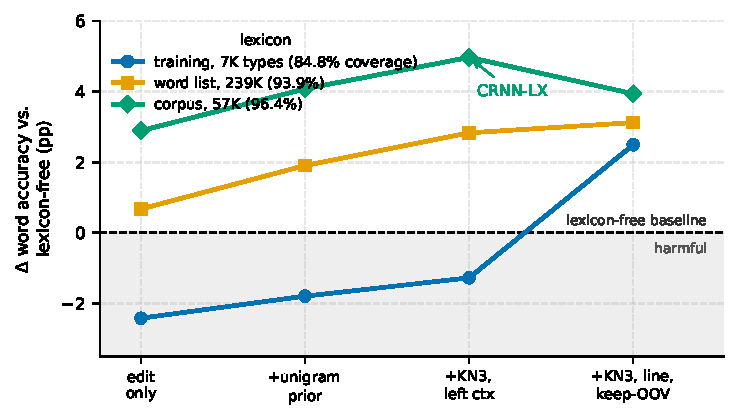
\includegraphics[width=\textwidth]{figures/fig4_lexicon_decomposition.pdf}}
\vspace*{8pt}
\caption{What the post-corrector contributes, measured against lexicon-free
decoding. (a) Coverage decides the sign: with 7\,K types both variants
fall below the baseline, with 239\,K both rise above it. The vertical
gap between the two lines is the contribution of the frequency prior,
and it doubles as the lexicon grows. Thick lines: the \ours\ optical
model; faint lines: the other five configurations of
Table~\ref{tab:main}. (b) Build-up on the 239\,K lexicon: edit distance
alone, the unigram prior, the Brown corpus, left-to-right line context,
and whole-line decoding with keep-OOV (white labels: increment over the
previous bar).}
\label{fig:lexdecomp}
\alttext{Two panels. Left: line chart of the change in word accuracy against lexicon size, with and without the frequency prior, relative to lexicon-free decoding. Right: five bars showing the cumulative gain of edit distance, unigram prior, Brown corpus, left-to-right context and whole-line decoding on the 239K lexicon.}
\end{figure}

The character error rate does not follow word accuracy. A whole-word
corrector can only replace a hypothesis by a complete lexicon entry;
when the replacement is wrong, a near-miss with one character error
becomes a different word with several. The training lexicon, which
replaces many correct-but-unlisted words, pays this price most heavily
(11.19\% against \rawcer\ lexicon-free); the extended lexicon with the
unigram prior pays it less (9.09\%) but still raises CER by half a
point while improving WA by almost two. Only the trigram on the larger
corpus chooses the right candidate often enough to bring CER back to
the lexicon-free level (8.58\% left to right, \ourcer\ with whole-line
decoding). Lexicon-assisted word accuracy and
character error rate therefore measure different things and should be
reported together.

\subsection{Comparison with Prior Word-Level Systems}
\label{sec:res-prior}

Table~\ref{tab:priorwork} places \ours\ next to seven published
word-level systems and states, for each, whether a lexicon or language
model was applied at test time. Three of our own rows are given,
because they answer different questions: \oursnolm\ is the optical
model alone; the \emph{no-context} row applies the extended lexicon
with the unigram prior and is the figure for words that are genuinely
isolated; \ours\ additionally reads the recognizer's own outputs for
the neighbouring crops of the line, which none of the listed systems
does. The upper block lists results obtained on the Aachen
writer-disjoint partition. The closest match in protocol is the
sequence-to-sequence recognizer of Sueiras et
al.~\cite{sueiras2018offline}: the sizes of their partition
(47\,952, 20\,306 and 7\,558 words, as compiled
in~\cite{mondal2022yolo}) are those of the \texttt{ok}-filtered Aachen
training, test and validation lists (47\,999, 20\,310 and 7\,559) from
which ours are drawn, and they report lexicon-free word and character
error rates on the full test partition exactly as we do. Under
lexicon-free decoding \oursnolm\ is 2.6\,pp more accurate (\rawwa\
against 76.20\%) at a slightly lower CER (\rawcer\ against 8.80\%);
with the extended lexicon the margin is 4.5\,pp without context and
5.8\,pp with it. \ours\ remains below the later attention-based
systems: 0.6\,pp below Kang et al.~\cite{kang2018convolve}, 2.1\,pp
below the candidate-fusion model of Kang et
al.~\cite{kang2021candidate} and 2.7\,pp below
AttentionHTR~\cite{kass2022attentionhtr}, which additionally transfers
knowledge from 14.4\,M scene-text images; without line context each
gap is 1.2\,pp wider (1.8, 3.4 and 3.9\,pp), and against our
lexicon-free figure 3.1\,pp wider. The gap is larger at character
level (5.79--6.88\% against our 8.54--8.60\%), consistent with the
autoregressive decoders of those systems modeling inter-character
dependencies that a CTC output with whole-word post-correction cannot.
The lower block reports three systems measured on other partitions of
IAM; \ours\ is above all three and \oursnolm\ above two, but the
partitions differ in writer overlap and size and we draw no conclusion
from margins of this size.

\begin{table}[th]
\tbl{Word-level results on IAM. WA in parentheses is derived as
$1-\mathrm{WER}$ from the cited paper. Lexicon: lexical constraint at
test time (none = unconstrained decoding; LM = language model without
a closed lexicon; n/s = not stated). Only \ours\ uses the recognizer's
outputs for the neighbouring crops of the line; every other row
recognizes each word in isolation.\label{tab:priorwork}}
{\begin{tabular}{llccc}
\toprule
System & Year & Lexicon & WA (\%) & CER (\%) \\
\colrule
\multicolumn{5}{l}{\emph{Aachen writer-disjoint partition ($\approx$20.3\,K test words)}} \\
Sueiras et al.~\cite{sueiras2018offline}      & 2018 & none & (76.20) & 8.80 \\
Kang et al.~\cite{kang2018convolve}           & 2018 & none & (82.55) & 6.88 \\
Kang et al.~\cite{kang2021candidate}          & 2021 & LM   & (84.09) & \textbf{5.79} \\
Kass and Vats~\cite{kass2022attentionhtr}     & 2022 & none & (\textbf{84.60}) & 6.50 \\
\oursnolm\ (ours)                             & 2026 & none & 78.83 & 8.60 \\
\ours, no context (ours)                      & 2026 & 239\,K $+$ unigram prior & 80.74 & 9.09 \\
\textbf{\ours} (ours)                         & 2026 & 239\,K $+$ trigram, line context & 81.95 & 8.54 \\
\colrule
\multicolumn{5}{l}{\emph{Other partitions of IAM}} \\
Mondal et al.~\cite{mondal2022yolo}\tabmark{a}                                    & 2022 & none & (70.79) & 9.53 \\
CNN--RNN of~\cite{dutta2018improving}, re-trained in~\cite{rajesh2022hwrcnet}\tabmark{b} & 2022 & n/s & (77.14) & 11.08 \\
Rajesh et al.~\cite{rajesh2022hwrcnet}\tabmark{b}                                 & 2022 & n/s & 80.08 & 9.89 \\
\botrule
\end{tabular}}
\begin{tabfootnote}
\tabmark{a} 30\,K randomly selected test words; 1\,200 training images.\\
\tabmark{b} Random 95:5 split, writer-dependent, $\approx$5.8\,K test words.
\end{tabfootnote}
\end{table}

\subsection{Error Analysis}
\label{sec:res-err}

\ours\ misrecognizes 3\,665 of the \nsamples\ test words. Only 275 of
them (7.5\%) differ from the reference in letter case alone; the
remaining errors are genuine. At character level the aligned errors
consist of 5\,219 substitutions, 1\,286 deletions and 486 insertions,
so the model drops characters far more often than it hallucinates
them. Fig.~\ref{fig:confusion} shows the ten most frequent
substitutions: they are mostly symmetric confusions between visually
similar lower-case glyphs --- \texttt{o}$\leftrightarrow$\texttt{a}
(257 cases in both directions), \texttt{s}$\leftrightarrow$\texttt{r}
(151), \texttt{n}$\leftrightarrow$\texttt{m} (107),
\texttt{t}$\leftrightarrow$\texttt{l} (101),
\texttt{n}$\leftrightarrow$\texttt{r} (90),
\texttt{e}$\leftrightarrow$\texttt{a} (87).
Case substitutions account for 7.8\% of all substitutions.
Of the post-corrector's decisions, 1\,925 hypotheses (9.5\%) are
replaced: 815 wrong hypotheses become correct and 181 correct ones,
valid words absent from the lexicon, become wrong. The left-to-right
decoder without keep-OOV replaces 2\,939, repairs 1\,076 and breaks
501; the unigram prior replaces the same 2\,939 and breaks the same
501 --- the lexicon decides which words are touched --- but repairs
only 888. Whole-line decoding with keep-OOV thus wins not by repairing
more but by leaving alone the words it would have broken. The
confusions themselves are errors of shape, not of vocabulary: a
whole-word lexicon can repair them
only when the mis-shaped word falls outside the lexicon and its correct
form lies within two edits, which is exactly the population that the
extended lexicon recovers in Table~\ref{tab:lexicon}.

\begin{figure}[th]
\centerline{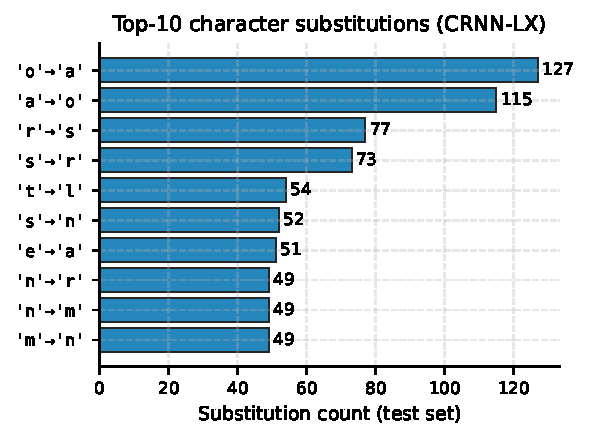
\includegraphics[width=9.2cm]{figures/fig3_confusion_topk.pdf}}
\vspace*{8pt}
\caption{Ten most frequent character substitutions of \ours\ on the
test set (true\,$\rightarrow$\,predicted).}
\label{fig:confusion}
\alttext{Horizontal bar chart of the ten most frequent character substitutions and their counts on the test set.}
\end{figure}

% ---- 6. Discussion ------------------------------------------------------
\section{Discussion}
\label{sec:discussion}

\subsection{Interpretation of the Augmentation Results}

The anchor rules out the explanation that would otherwise be hardest
to exclude. A null result can always mean that the experiment is too
noisy to see anything, and the seed repeats confirm that the noise is
real: an unchanged configuration moves by a full point from seed to
seed. But the same test, the same data and the same protocol detect the
removal of the conventional pipeline at $p=1\times10^{-30}$, 2.7
points of word accuracy. The apparatus is not blind to augmentation; it
cannot resolve \emph{these} transforms on \emph{this} training set,
whose largest effect ($+0.32$\,pp, $p=0.132$) stays below the
threshold, changes with the post-corrector ($+0.44$\,pp, $p=0.025$
under the left-to-right corrector) and changes sign with the seed
(Table~\ref{tab:seeds}). What we observe is consistent with
saturation, and three further observations indicate where it occurs.

First, the anchor overfits earliest and hardest: at epoch 53, where it
stops, its training loss is 0.018 against 0.056--0.070 for the
augmented runs, and its validation loss has risen $0.10$ above its own
minimum, against $0.03$--$0.07$ for them; the augmented runs stop 32 to
47 epochs later (Fig.~\ref{fig:curves}). The first increment of
augmentation buys regularization that the network genuinely needs. Second, among the
augmented configurations the validation curves coincide and the extra
transforms neither slow convergence nor raise the plateau, while the
fully augmented model reaches a slightly higher training loss --- so
they do regularize further, but the baseline is no longer overfitting
in a way that costs accuracy on unseen writers. Third, the per-word
disagreements between those configurations are large yet balanced.
Together these indicate that with 48\,K training words from 283
writers, the writer-to-writer variation already present in the data
exceeds what elastic and morphological perturbation of 64-pixel-high
crops can add on top of affine and photometric jitter. Reports of
sizeable gains from such augmentation, including our own preliminary
experiments, came from smaller training sets or from comparisons in
which augmentation was not the only difference. The result does not
imply that augmentation is useless for HTR in general --- Wigington et
al.~\cite{wigington2017data} report gains on lines with a different
transform family, and our own anchor shows the first increment is
worth 2.7\,pp --- but it does show that further transforms must be
measured under controlled conditions before being claimed.

\subsection{Coverage and the Frequency Prior}
\label{sec:disc-lex}

The ablation separates four effects that are usually conflated under
``adding a language model'', and they turn out to do different jobs.
Membership testing against a list that covers 85\% of the test tokens
is harmful, because the corrector cannot distinguish a misrecognized
word from a correctly recognized word it has never seen and treats
both as errors; raising coverage to 94\% is what turns the loss into
a gain. That gain is small on its own, however. What converts it into
$+1.9$\,pp is the prior that ranks the candidates, and it is worth
twice as much on the large lexicon as on the small one.

The unigram prior is not doing linguistic work; it breaks ties. The
tighter the lexicon, the fewer entries lie within two edits of a
hypothesis and the less the ranking matters; at 239\,K types a
mis-shaped word typically has several equidistant neighbours, and
picking the frequent one is right more often than picking an arbitrary
one. Edit distance identifies the candidate set and frequency chooses
inside it: reporting either without the other describes only half of
the corrector.

The trigram does linguistic work, but only once it has text to learn
it from. On the 48\,K tokens of IAM training text the line context is
worth $0.10$\,pp, because the two words preceding a test word rarely
form a context the model has seen; on 1.2\,M tokens it is worth
$0.34$\,pp, and the corpus itself, even without context, is worth
$0.59$\,pp, because 7\,K types observed once or twice give a poor
estimate of which of two candidates is the commoner English word.
Decoding the line jointly adds another $0.29$\,pp, but the larger part
of that comes from a different mechanism than context: letting an
unlisted hypothesis survive turns the corrector from one that must
replace every unlisted word into one that may, and the line objective
then decides. The left-to-right corrector broke 501 correctly
recognized words that the lexicon did not contain; the whole-line
decoder breaks 181 (Section~\ref{sec:res-err}). The ceiling is close:
the corrector only ever touches the 16\% of hypotheses that fall
outside the lexicon, and with reference transcriptions as context the
left-to-right corrector gains a further $0.06$\,pp only. What remains
after correction is therefore not a ranking problem. The character
error rate confirms the division of labour: the unigram corrector buys
word accuracy at the price of character accuracy (9.09\% against
8.60\% lexicon-free), because a wrong whole-word substitution turns a
near miss into several character errors. The trigram replaces exactly
the same hypotheses but picks the right candidate for 1\,076 of them
instead of 888, and ends at the lexicon-free value (8.58\% left to
right, \ourcer\ whole-line).

A practical consequence is that word-level HTR results obtained with a
closed lexicon should state the lexicon's coverage of the test
vocabulary, the rule used to rank candidates, the corpus the ranking
was learned from and whether any context was used, without which the
reported accuracy is not interpretable. The remaining 6\% of uncovered
tokens (proper nouns, rare inflections, punctuation-bearing strings)
bound what any whole-word corrector can achieve; addressing them
requires an open-vocabulary character-level model.

\subsection{Comparison with Previous Word-Level HTR Systems}
\label{sec:disc-sueiras}

Among the systems of Table~\ref{tab:priorwork}, the recognizer of
Sueiras et al.~\cite{sueiras2018offline} is the one whose protocol
matches ours most closely: isolated
IAM words, the Aachen writer-disjoint partition drawn from the same
\texttt{ok}-filtered word lists --- the only prior system for which we
could verify this from the reported partition sizes
(Section~\ref{sec:res-prior}); we additionally discard two unreadable
images and five validation forms whose prompts recur in the test
set --- and lexicon-free word and character error rates on the full
test partition. Architecturally the two differ in every stage: they extract features from a sliding window
of image patches with a LeNet-5-style convolutional network and
transcribe them with a recurrent encoder--decoder using attention,
whereas \oursnolm\ is a single convolutional-recurrent network trained
with CTC. Under lexicon-free decoding \oursnolm\ reaches \rawwa\
against their 76.20\% (23.8\% word error rate), a margin of 2.6\,pp
that is almost five times the half-width of our confidence interval,
at a slightly lower character error rate (\rawcer\ against 8.80\%).
Post-correction with the extended lexicon widens the word-level margin
to 4.5\,pp without context and 5.8\,pp with it. Sueiras et al. also report lexicon-constrained variants of
their recognizer; those depend on the lexicon employed and are not
compared here. We read the comparison as evidence that a plain CRNN
trained from scratch on the 48\,K Aachen training words is competitive
with an early attention model under the same protocol, not as evidence
about augmentation: the proposed transforms contribute nothing
measurable to that margin (Tables~\ref{tab:main}
and~\ref{tab:seeds}).

HWRCNet~\cite{rajesh2022hwrcnet}, the closest system in construction
(a CNN, a bidirectional LSTM and a CTC layer), reports 80.08\% strict
word accuracy, 1.87\,pp below \ours\ (0.66\,pp below its no-context
variant) and 1.25\,pp above \oursnolm. It
is measured on a random 95:5 partition whose test set is
writer-dependent and about 3.5 times smaller than ours, so neither
difference is interpretable.

\subsection{Threats to Validity}

The augmentation differences of 0.1--0.3\,pp are below what one
training run can resolve: with three seeds the CRNN-B--\ours\
difference changes sign and averages $+0.20\pm0.64$\,pp
(Table~\ref{tab:seeds}), so we report the transforms as unresolved
rather than as small gains. Only the two endpoint configurations were
repeated; the four intermediate ones were trained once, and their
individual $p$-values in Table~\ref{tab:main} therefore carry no more
weight than the seed-42 row of Table~\ref{tab:seeds} does. The
repeats also ran on different hardware, so the spread we quote
includes any hardware-related nondeterminism --- which only reinforces
the conclusion that an effect of this size is not resolvable here.
The \anchordelta\,pp effect of the conventional pipeline is an order of
magnitude larger than that resolution limit, so the positive control
does not depend on the seed in the way the null result does.
The lexicon and ranking effects ($-2.4$ to $-2.7$\,pp for the
training vocabulary, $+1.1$ to $+1.3$\,pp for the frequency prior) are
reproduced in sign and ordering on all six independently trained
models and are well outside the interval, although their magnitude
grows as the optical model weakens. The gain of the left-to-right
trigram over the unigram prior is equally stable: $+0.85$ to
$+0.96$\,pp on each of the six optical models, with $\alpha=7$ selected
on validation for all of them; whole-line decoding then adds $+0.29$
to $+0.44$\,pp on the five augmented models and $+0.08$\,pp on the
anchor. The whole-line decoder has two options and a wider penalty
grid, all selected on the 7\,205 validation words; a variant that was
not selected (real-word substitution) reaches almost the same test
accuracy by a different route, which shows that the selection is not
finely tuned to the test set but also that the validation set cannot
separate the two. These effects are, however, measured
with one candidate generator and one word list; a different
edit-distance bound or a different general vocabulary would change
their size, though the ordering of the post-corrections is unlikely to
change.
Validation accuracy, which the training loop measures with the unigram
corrector, exceeds the test accuracy of that same corrector by about
four points for every configuration; the validation writers are used
for checkpoint selection and are only 55 in number, so this gap is
expected and does not indicate a fault. The external systems in Table~\ref{tab:priorwork}
were trained and evaluated by their authors with their own
preprocessing and, in the lower block, on a different partition; we
therefore treat only our own runs as a controlled comparison. The extended lexicon is a general English word list and
contains no IAM test transcriptions, but it is a closed lexicon
nonetheless, and \ours\ should be read as a lexicon-assisted result.
Two further caveats concern the trigram. Its corpus is external to
IAM; we measured the verbatim overlap with the test lines
(Section~\ref{sec:trigram}) and found idioms only, but a corpus with
the same content as the prompts would inflate the result, and any
replacement corpus should be checked the same way. And its context is
the recognizer's output for the neighbouring crops, which exists
because IAM word images are cut from lines; on a collection of
genuinely isolated words the applicable figure is the no-context row
of Table~\ref{tab:priorwork} (\uniwa), not \ourwa. The edit penalty,
the decoder and its options were selected on the validation writers
and applied once to the test set.

% ---- 7. Conclusion ------------------------------------------------------
\section{Conclusion}
\label{sec:conclusion}

\ours\ recognizes handwritten words with \ourwa\ accuracy (\ourcer\
character error rate) on the complete Aachen writer-disjoint test set
of IAM, with a plain CRNN trained from scratch, no external image data,
and a post-corrector whose only external resource is a public text
corpus. Under the same partition and lexicon-free decoding the optical
model is 2.6\,pp more accurate than the sequence-to-sequence
recognizer of Sueiras et al.~\cite{sueiras2018offline}; the complete
system is 0.6--2.7\,pp below the later attention-based systems listed
in Table~\ref{tab:priorwork}, and 1.8--3.9\,pp below them when the
words are treated as isolated. Under controlled conditions, elastic
deformation, morphological perturbation and a
widened photometric range produce no statistically detectable change
in these figures --- over three seeds their apparent effect changes
sign and averages $+0.20\pm0.64$\,pp --- while removing the
conventional augmentation pipeline beneath them costs
\anchordelta\,pp, a pattern consistent with the benefit of
augmentation saturating before the transforms we proposed; a widely used elastic parameterization, moreover, does not
deform the image at all. The post-correction stage, by contrast, moves
accuracy by two to three points in either direction, and its four
ingredients do different jobs: the lexicon's coverage of the test
vocabulary decides whether the correction helps or hurts; the
frequency prior that ranks the candidates supplies most of the gain
once coverage is sufficient; an external corpus improves that ranking
further; and the line context, read from the recognizer's own outputs
on both sides of a word by decoding the line jointly, adds the last
$0.6$\,pp and returns the character error rate to the lexicon-free
level.

For word-level HTR the practical conclusions are that augmentation
gains should be demonstrated, not assumed, on the full training set;
that an ablation reporting no effect should include the configuration
in which the effect is known to exist, and should report the
run-to-run spread of an unchanged configuration, which at this scale
exceeded every augmentation effect we measured; that lexicon
coverage, the ranking rule, its corpus and its context should be
reported separately alongside lexicon-assisted accuracy; and that word
accuracy and character error rate should be given together whenever a
whole-word corrector is used. Future work will test whether the
augmentation becomes useful in the low-data regime, replace the
whole-word corrector with a character-level open-vocabulary model to
address the uncovered 6\% of tokens, and decode the line over the
optical model's full output distributions rather than over its
single-best hypotheses, so that the language model can also weigh
alternatives the greedy decoder discarded.


\section*{Acknowledgments}
We thank the maintainers of the IAM Handwriting Database and of the
Aachen split.

\bibliographystyle{ws-ijprai}
\bibliography{references}

\end{document}
